\documentclass[11pt]{article}
\usepackage[a4paper,margin=2.5cm]{geometry}
\usepackage{graphicx}
\usepackage{booktabs}
\usepackage{amsmath}
\usepackage{hyperref}
\usepackage{xcolor}

\title{NexaFreight: A Validation-Gated Multimodal Freight Control Tower\\
for India-Anchored Logistics\\[4pt]
\large Reproducible decision support where no public ground truth exists}
\author{Raj Montana\\
\small Independent research project (rebuild series, days 1--13)\\
\small \texttt{github.com/rajmontana/NexaFreight}}
\date{September 24, 2026}

\begin{document}
\maketitle

\begin{abstract}
Enterprise control towers promise end-to-end visibility and re-optimization,
yet no public multimodal shipment dataset exists to train, benchmark, or
audit such systems. We present NexaFreight, an open, India-anchored freight
control tower whose central claim is methodological: \emph{when ground truth
is unavailable, every operational number must either trace to a published
reference or carry an explicit provenance label}, and this rule must be
enforced by CI, not convention. The system implements a schedule-aware
multimodal planner (four single-objective scalarizations plus Yen
$k$-shortest paths over a time-expanded graph, scored by priority-profile
weights), quantile ETA regression (LightGBM p10/p50/p85) with
champion-guard retraining and drift monitoring, a financial engine with
pinned SLA/demurrage/carbon constants, an event-driven
disruption--alert--decision loop with immutable audit and revealed-choice
preference learning, and a deterministic synthetic world generator for
reproducible demonstration. A 37-check validation matrix (30 static
published references + 7 committed artifact checks) gates every commit;
measured Suez-vs-Cape diversions (1.70/1.73/1.25 distance ratios on the
searoute marine graph) reproduce UNCTAD-anchored reporting bands inside a
CI drill. We document an audited train/serve skew found and closed in the
feature contract, a capacity-blind consolidation defect corrected to
ISO~668 tonnage arithmetic, and a correction path from synthetic to real
data (PortWatch, Open-Meteo, AISStream, ULIP) that leaves the engine
unchanged. The full stack, test suites (538 unit / 184 integration), and
paper figures are reproducible from a clean clone.
\end{abstract}

\section{Introduction}

Freight operators increasingly adopt \emph{control towers}: layered
visibility-and-decision systems above execution systems (TMS/WMS). The
domain literature and practitioner surveys describe the control-tower
pattern as event-driven visibility, exception triage by business loss,
and re-optimization with human-in-the-loop approval. Academic treatments
of dynamic vehicle routing similarly emphasize event-triggered
re-optimization with hysteresis to prevent plan churn.

Building and \emph{auditing} such a system outside a company, however,
collides with a data wall: to our knowledge no public dataset pairs
multimodal shipments (sea/air/rail/road), milestones, costs, disruptions,
and decisions. Public datasets are either single-mode (AIS traces, flight
tracks), single-actor (a carrier's EDI events), or historical
macro-statistics. This is the unsolved problem NexaFreight addresses
methodologically rather than by pretending the data exists.

\textbf{Contributions.}
\begin{enumerate}
\item \textbf{A validation-gated architecture}: a 37-check matrix that
compares every financially and operationally consequential constant
against published references (GLEC emission factors, UNCTAD-anchored
diversion reporting, Indian Railways freight statistics, World
Bank/PortWatch dwell ranges, ISO 668 container capacities), executed in
CI on every push; plus row-level provenance (REAL/DERIVED/SIMULATED)
surfaced in the analytics API so blended provenance cannot hide.
\item \textbf{A complete multimodal decision loop}: time-expanded
schedule-aware planning with capacity and connection constraints; a
disruption detector (congestion ratio tiers); ranked reroute options
priced in USD and kg CO$_2$; approval-gated execution with immutable
decision audit; outcome finalization feeding revealed-choice preference
learning and champion-guard model retraining.
\item \textbf{Quantile ETA prediction with governance}: p10/p50/p85
LightGBM boosters, one shared feature contract for train and serve (an
audited train/serve skew is documented and closed with a sentinel
unification and a prediction-equality test), drift monitoring, and
preference-band demotion.
\item \textbf{A deterministic synthetic world} (seeded RNG, calibrated to
published Indian logistics statistics) that makes every figure in this
paper reproducible from a clean clone, including an India export-chain
party model (shippers, consignees, carriers) and tonnage-true container
arithmetic.
\item \textbf{An honest substitution roadmap}: seam-by-seam replacement
of synthetic inputs with open data (PortWatch, Open-Meteo/ERA5, AISStream,
ORS/OSM rail graphs, EM-DAT) and the production path (India's ULIP),
written so that each swap touches data only --- never the engine.
\end{enumerate}

We position this as an engineering-methods contribution: the reusable
idea is the \emph{validation gate + provenance + deterministic demo}
triad for auditing decision-support systems in domains without public
ground truth.

\section{System architecture}

NexaFreight is a two-tier system. A FastAPI/SQLAlchemy backend owns the
operational state in a relational schema (locations, network nodes/edges/
schedules, shipments, orders, legs, positions, ports and daily port
statistics, disruptions, alerts, decisions, decision outcomes,
corridor alternatives, users, and a parameter table). A Next.js frontend
renders a live control tower: a tactical globe with per-mode route layers
and moving markers fed by a server-sent-events position stream, ops
panels (financial scorecard, SLA board, ESG rail, alerts), a public
/validation page rendering the live check matrix, and an ops copilot
endpoint with a rule-based fallback.

Three cross-cutting invariants hold throughout:
\begin{enumerate}
\item \textbf{Single source of parameters.} Speeds, cost rates, emission
factors, thresholds, planner policy, and business constants load from a
\texttt{parameter\_empirical} table (51 keys cached at boot) with a
committed fallback registry; inline shadow defaults were removed in an
audited cleanup after two subsystems were found carrying
\emph{different} implicit values for the same key.
\item \textbf{Provenance on rows.} Operational rows carry
REAL/DERIVED/SIMULATED provenance; analytics roll up per-provenance
buckets so bake-era template plans and runtime planner output are never
silently blended.
\item \textbf{Everything gated.} Beyond unit/integration suites and
typecheck, CI runs the 37-check validation matrix and a scripted Red Sea
disruption drill on every push.
\end{enumerate}

\section{Methods}

\subsection{Route planning and optimization}

The network is a time-expanded multimodal graph: physical edges carry
distance, reliability, and parameter keys (speed, cost rate, CO$_2$
intensity); timetable departures make waiting and transfers first-class.
For a shipment with tonnage $W$, each leg of candidate itinerary $\pi$
receives
\begin{align}
\mathrm{cost}(\pi) &= \sum_{e \in \pi} d_e \, c_e \, W,\\
\mathrm{co}_2(\pi) &= \sum_{e \in \pi} d_e \, f_e \, W / 1000,\\
\mathrm{time}(\pi) &= \text{timetable-derived transit and wait hours},\\
\mathrm{rel}(\pi) &= \prod_{e \in \pi} r_e .
\end{align}
The planner runs four single-objective scalarizations (cost, time,
CO$_2$, reliability) as label-setting searches on the time-expanded
graph, adds Yen $k$-shortest paths on the cost weighting for diversity,
prunes infeasible candidates (missed connections below the
\texttt{connection\_margin} policy; deadlines impossible), and scores
survivors with a normalized weighted objective
$\sum_m w_m \hat{v}_m$ whose weights are priority profiles
(CRITICAL/EXPRESS/STANDARD/ECONOMY) from the parameter table. The top-$k$
ranked itineraries are returned; the approved option is executed as leg
rows with immutable decision audit, and observed approvals feed a
revealed-choice preference model that demotes repeatedly rejected option
families in future slates (no hand-tuned learning weights).

\subsection{Quantile ETA, delay risk, and governance}

ETA is LightGBM quantile regression: three boosters predict
p10/p50/p85 of shipping days from a versioned feature contract
(mode, cargo class, revenue/cost ratios, scheduled days, geography,
calendar features, distance/leg-count, and congestion features wired for
the next training generation). p85 is the promise date used by the SLA
checker; the delay classifier supplies the ML path of SLA risk scoring
with a rule-based fallback (availability over correctness, logged).
Governance: a challenger retrains behind a champion guard requiring
$\ge 0.5\%$ relative improvement in mean test pinball loss; a drift
monitor watches artifact age and input row change; the committed champion
reports test pinball 0.9345 with a rearrangement sanity check of 1.0.
A committed skew test proves train-path and serve-path encodings produce
identical frames and identical booster predictions on committed rows:
the audit had found train-side unseen categoricals becoming NaN while
serve-side mapped them to a sentinel; both now share one encoder.

\subsection{Financial engine}

Realized and projected financials compose from pinned constants:
freight as summed executed-leg costs (distance $\times$ rate $\times$
tonnes; tonnage from measured order weights with ISO 668-derived
container arithmetic, 28{,}000\,kg / 33\,m$^3$ per twenty-foot
equivalent); SLA penalty at 5\%/day of order revenue capped at 10\% (a
documented planning multiplier $\approx$7$\times$ late-delivery norms,
not a market quote); demurrage at 4 free days then USD~62.5/day with a
$\times$2 tier after day 7; carbon as tonne-km $\times$ mode emission
factor (GLEC-calibrated sea 8.0 g/t-km) $\times$ a pinned carbon price.
Analytics roll these into cumulative day/week/month windows and
per-provenance buckets; every constant either traces to a reference in
the validation matrix or is labeled a documented planning assumption.

\section{The validation-gate methodology}

\subsection{Matrix design}

The gate (37 checks: 30 static + 7 committed artifacts) is a plain
service consumed by three surfaces --- a CLI gate in CI, a public API
endpoint, and a dashboard page --- so the screen can never disagree with
CI. Static checks pin published values within tolerances; artifact
checks recompute committed model metrics and drill outputs. Spot
examples: per-port dwell medians (e.g., JNPT p50 $= 22.0 \pm 2.0$ h
against India all-vessel reporting with a one-sided bound at 48.84 h),
GLEC sea EF $8.0$ g/t-km (band 7.6--9.1), Indian Railways class-average
freight in INR/t-km, ISO 668 container payload/volume, congestion alert
tiers (1.5$\times$/2.5$\times$ against PortWatch-methodology
plausibility), and Cape diversion ratios within UNCTAD-anchored bands.

\subsection{Provenance discipline}

The demo world is deterministic (seeded RNG across world-build and
order-drip; identical rebuilds reproduce identical party assignments,
loads, and itineraries). Every synthetic row is labeled; the analytics
API exposes per-provenance financial buckets; the map renders
provenance badges on telemetry. The claim \emph{``no uncalibrated
number reaches the screen''} is enforced by code, and the enforceability
itself is the contribution.

\section{Results}

\subsection{Measured corridor responses (Red Sea scenario)}

Table~\ref{tab:corridor} reports searoute-measured Suez vs.\ Cape of
Good Hope diversions for the three scripted lane groups (neo-panamax),
all inside the UNCTAD-anchored reference bands; the same measurements
seed the corridor alternatives used by the reroute engine and run as a
CI drill on every push.

\begin{table}[h]
\centering
\begin{tabular}{lrrrr}
\toprule
Lane & Suez (nm) & Cape (nm) & ratio & added hours\\
\midrule
INJNP$\rightarrow$NLRTM & 6{,}380 & 10{,}848 & 1.70 & $+198.8$\\
INMUN$\rightarrow$NLRTM & 6{,}366 & 11{,}045 & 1.73 & $+208.8$\\
SGSIN$\rightarrow$NLRTM & 8{,}383 & 10{,}441 & 1.25 & $+84.0$\\
\bottomrule
\end{tabular}
\caption{Measured VIA\_CAPE diversion factors (searoute marine graph,
neo-panamax). References: India--EU $1.72\pm0.15$,
Singapore--EU $1.25\pm0.08$.}
\label{tab:corridor}
\end{table}

\begin{figure}[h]
\centering
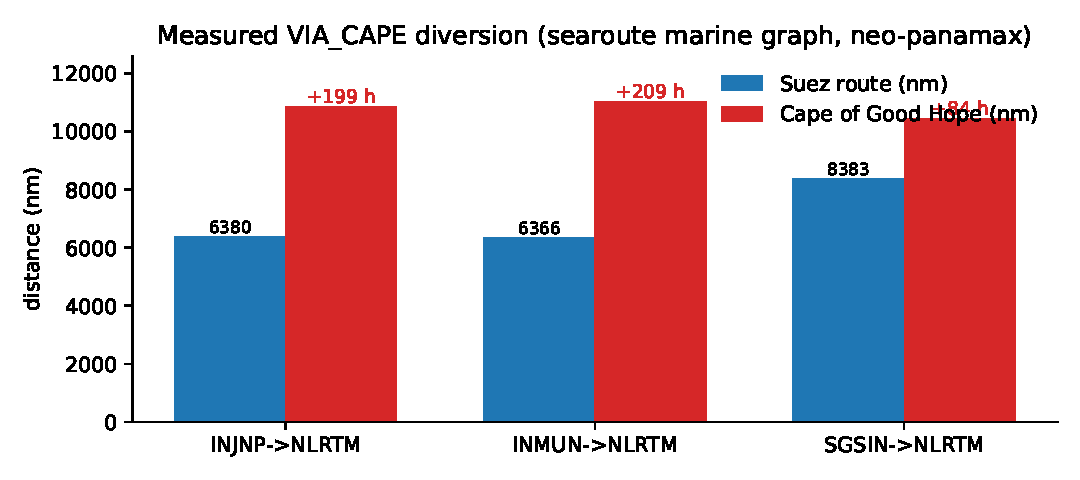
\includegraphics[width=.85\linewidth]{figures/fig_corridor.pdf}
\caption{Measured Suez vs.\ Cape distances per lane group with added
transit hours.}
\end{figure}

\subsection{Validation matrix composition}

\begin{figure}[h]
\centering
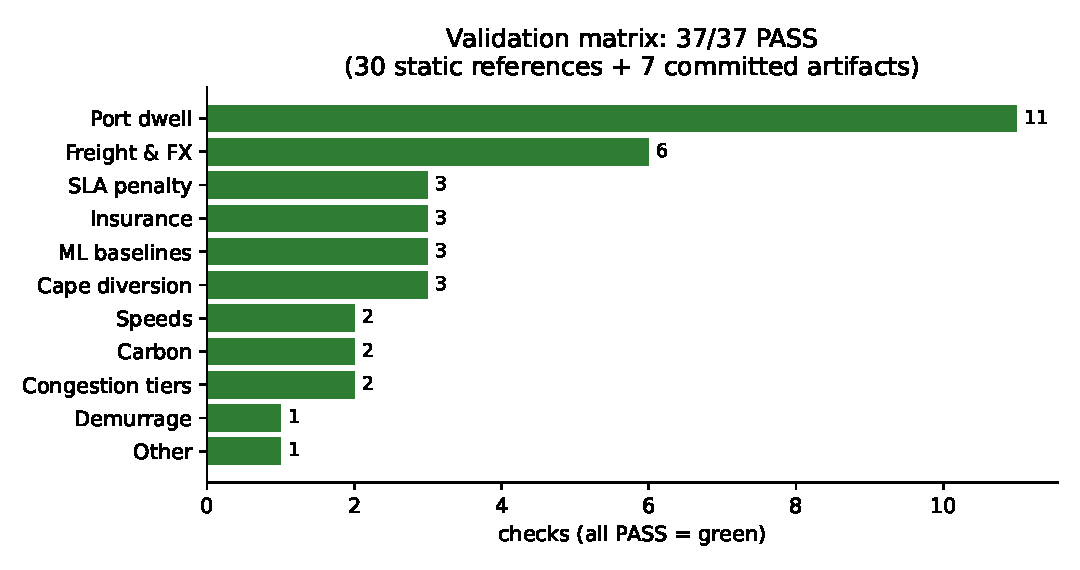
\includegraphics[width=.85\linewidth]{figures/fig_validation_matrix.pdf}
\caption{The 37-check validation matrix by category; all checks PASS on
the frozen commit. Failure of any check fails CI.}
\end{figure}

\subsection{Mode emission factors}

\begin{figure}[h]
\centering
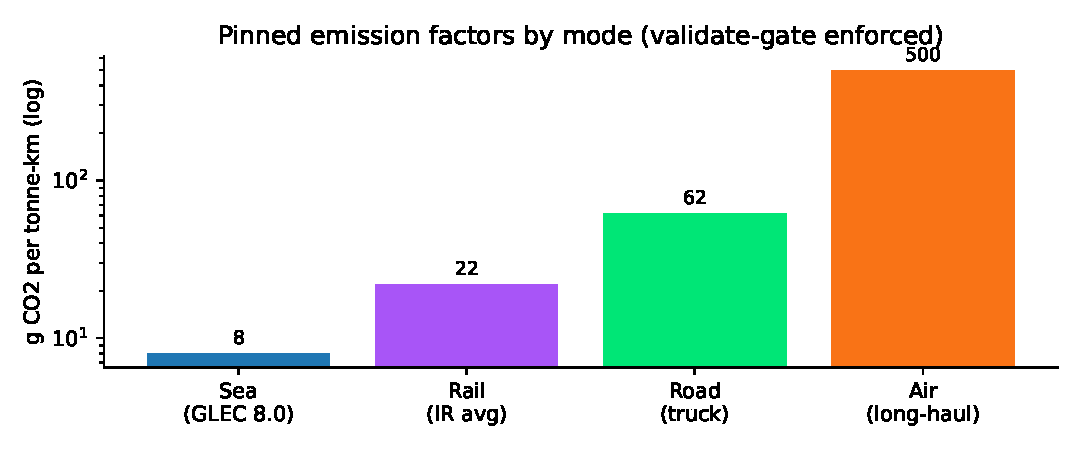
\includegraphics[width=.85\linewidth]{figures/fig_mode_co2.pdf}
\caption{Pinned emission factors (log scale). Sea is GLEC-calibrated;
rail reflects Indian Railways diesel-era averages --- an
electrification-blended refinement is future work.}
\end{figure}

\subsection{Committed model metrics}

On the committed DataCo test split, the delay classifier reports
accuracy 0.7313, precision 0.7911, Brier 0.2326; the ETA model reports
test pinball p10/p50/p85 $= 0.1685 / 0.5054 / 0.2562$ against a grouped
quantile baseline p85 pinball of 0.2080 (sea-inclusive split). These are
artifact checks in the validation matrix, not claims of
state-of-the-art: the contribution is that the numbers are \emph{pinned,
reproducible, and skew-audited}, with governance to replace them.

\subsection{Audited defects and corrections}

Three representative defects found by the process, each fixed with a
regression test: (i) \textbf{train/serve skew} --- unseen categorical
levels encoded differently across paths; closed by one shared encoder
plus prediction-equality tests. (ii) \textbf{Capacity-blind
consolidation} --- container counts from order tallies
($\lceil n/20\rceil$ and, worse, $n$) in two code paths; replaced by
binding-dimension arithmetic on measured weight/volume with
cargo-class nominals as documented fallback (90\,t on one order now
prices 4 TEU-equivalents). (iii) \textbf{Shadow parameter defaults} ---
the planner and world builder carried different implicit values for the
same key; unified into the registry with a guard test. A fresh-clone
corridor-seeding crash (missing foreign port coordinates on machines
without gitignored ingest files) and a map layer that rendered rail
assets with flight glyphs were additionally found by external
machine-specific runs and fixed with tests.

\subsection{End-to-end gates at freeze}

Unit 538 passed +2 skipped (environment-dependent model-artifact
skips); integration 184 passed; TypeScript clean; 239 frontend tests;
validation matrix 37/37; Red Sea drill GREEN in CI. The demo world at
freeze: 9 parties, 50+ shipments across all four modes, 1{,}092 port-day
observations, deterministic under rebuild.

\section{Reproducibility}

The repository is public. A clean clone applies an ordered
format-patch series (or pulls merged main), runs Alembic to head,
rebuilds the deterministic world (one command, $\approx$4--6 min), and
reproduces every gate and figure; CI executes the validation gate and
disruption drill on every push without secrets. All paper figures are
generated by a committed script from the live validation service and
measured artifacts. No API key is required for any reported result;
external integrations degrade to documented fallbacks.

\section{Limitations and data availability}

\textbf{The corpus is synthetic and says so.} No lawful public source
exists for multimodal shipment streams with outcomes; NexaFreight
therefore trains on a public single-actor e-commerce dataset (DataCo)
plus a calibrated synthetic world whose rates (dwell, speeds, costs,
congestion) are themselves reference-validated. The synthetic corpus is
a demonstration and benchmarking substrate, not a market sample.

\textbf{Planned substitutions (engine unchanged).} PortWatch (World
Bank) port-call/waiting-time data replaces simulated port statistics and
closes two open calibration questions (per-port dwell tails; congestion
tier plausibility); Open-Meteo/ERA5 instantiate the designed weather
delay factor; AISStream supplies live vessel positions behind the
existing env-gated adapter; ORS or self-hosted OSRM and OSM rail-graph
extraction (osmnx; or the Geofabrik OpenRailRouting engine) replace
straight-line road/rail geometry; EM-DAT provides disruption priors;
India's ULIP is the production integration path for real orders and
milestones. Each seam ingests nightly into existing tables with
provenance REAL; nothing external sits in a request path.

\textbf{Known frozen-issue.} A legacy ingest-era parameter row for sea
CO$_2$ intensity (6.5 g/t-km) predates the GLEC-calibrated pin (8.0);
financial mathematics use the pinned value, and the row is queued for
regeneration in the first post-freeze pass.

\section{Conclusion}

Where ground truth does not exist, auditability must be manufactured.
NexaFreight demonstrates that a full multimodal control tower ---
planning, prediction, event-driven re-optimization, financials,
governance --- can be built so that \emph{every number is either
referenced, measured, or labeled}, and that this property can be
enforced continuously by CI at zero external-dependency cost. The
engineered seams let real data replace synthetic inputs without
touching the engine, which is the practical path from an honest demo to
an operational system.

\begin{thebibliography}{9}
\bibitem{glec} Smart Freight Centre. \emph{Global Logistics Emissions
Council (GLEC) Framework v3.x} --- logistics emissions accounting
methodology; sea EF guidance band. \url{https://www.smartfreightcentre.org}
\bibitem{unctad} UNCTAD, \emph{Review of Maritime Transport 2024} and
contemporaneous shipping-market commentary on Red Sea diversions
(distance/time impact reporting). \url{https://unctad.org}
\bibitem{portwatch} World Bank / International Monetary Fund.
\emph{PortWatch}: port calls, waiting times, and trade disruption
monitoring from AIS. \url{https://portwatch.imf.org}
\bibitem{cppi} World Bank. \emph{The Container Port Performance Index
2023--2024}. \url{https://www.worldbank.org}
\bibitem{ir} Indian Railways / DFCCIL. Freight freight-rate class
averages and Dedicated Freight Corridor program statistics.
\url{https://dfccil.com}
\bibitem{iso668} ISO 668:2020. \emph{Series 1 freight containers ---
classification, dimensions and ratings} (20 ft: 30{,}480 kg max gross).
\bibitem{dataco} Souza, A.M. et al. (2018). \emph{DataCo Smart Supply
Chain for Big Data Analysis} (public e-commerce logistics dataset,
Mendeley Data V4).
\bibitem{searoute} searoute-py: shortest sea routes on an OSM-based
marine network. \url{https://github.com/gis-ops/searoute}
\bibitem{yen} Yen, J.Y. (1971). Finding the $k$ shortest loopless paths
in a network. \emph{Management Science} 17(11).
\bibitem{lightgbm} Ke, G. et al. (2017). LightGBM: A highly efficient
gradient boosting decision tree. \emph{NeurIPS}.
\bibitem{pinball} Koenker, R., Bassett, G. (1978). Regression
quantiles. \emph{Econometrica} 46(1).
\bibitem{ulip} National Industrial Corridor Development / Government of
India. \emph{Unified Logistics Interface Platform (ULIP)}.
\url{https://ulip.nic.in}
\bibitem{openrail} Geofabrik. \emph{OpenRailRouting}: railway routing on
OpenStreetMap data with GraphHopper.
\url{https://github.com/geofabrik/OpenRailRouting}
\bibitem{emdat} EM-DAT: The International Disaster Database, Centre for
Research on the Epidemiology of Disasters (CRED).
\url{https://www.emdat.be}
\end{thebibliography}

\end{document}
